\typeout{------------------------------------------------------------------}
\typeout{} 
\typeout{        Fichier de base modifie par : Matth: 20 nov 2012} 
\typeout{                   sous licence GNU-GPL} 
\typeout{}
\typeout{------------------------------------------------------------------}

% Classe g�n�rale du document
   \documentclass[12pt]{report} % .10pt, 11pt, 12pt : taille de la police principale (10 par d�faut)
                 % .a4paper, letterpaper,... : d�limite la taille du papier. (letterpaper par d�faut)
	         % .fleqn : aligne les formules math�matiques � gauche au lieu de les centrer.
		 % .leqno : place la num�rotation des formules � gauche plut�t qu'� droite.
		 % .twocolumn : demande � LATEX de formater le texte sur deux colonnes.
		 % .twoside, oneside indique si la sortie se fera en recto-verso ou en recto simple.
		 % .landscape, mais il faut mettre en commentaire (ou modifier) toutes les dimmensions

% Importation de packages divers
%   \NeedsTeXFormat{LaTeX2e} 
   \usepackage[T1]{fontenc}
   \usepackage[utf8]{inputenc}		% utilisation des caract�res 8 bits en Unix (codage ISO 8859-1)
  %\usepackage[latin1]{inputenc}	% utilisation des caract�res pour Linux2
	\usepackage{color}
   \usepackage{fancyhdr}
   \usepackage{lastpage}
                   % pour l'affichage du n� de la derni�re page.
   \usepackage{lmodern}
   \usepackage{multirow}                % pour l'utilisation de figures ``noy�es'' dans le texte
   \usepackage{xspace}			% package pour babel
   \usepackage[english]{babel}         % Utilisation du fran�ais (nom des sections, c�sure, ponctuation,...)
   \usepackage{amsmath,amsthm,amssymb}  % Utilisation de certains packages de AMS (cf. belles �quations)
   \usepackage{endnotes}                % Pour l'utilisation des notes en fin de documents
   \usepackage{verbatim}                % Pour l'insertion de fichier en mode verbatim
   \usepackage{portland}		% pour l'utilisation de \portrait et de \landscape sur une page
   \usepackage[pdftex]{graphicx}        % [pdftex] si utilisation d'images jgp,...
                                        % [dvips]  si utilisation d'images bmp,...
   \usepackage{pdfpages}		% Inclure des pages de pdf
   \usepackage{setspace}		% Pour d�finir un interligne
   \usepackage[bottom]{footmisc}        % Footnote at the bottom
%   \usepackage[cyr]{aeguill}		% Pour les guillemets � la Fran�aise
   \usepackage{eurosym}	
   \usepackage{listings}
\usepackage{url}
\usepackage{setspace}
\urlstyle{sf}
	
   \renewcommand{\contentsname}{Summary} % si tableofcontents au d�but
   \newcommand{\Numero}{\No}
   \newcommand{\numero}{\no}
%   \newcommand{\fup}[1]{\up{#1}}

   \DeclareGraphicsExtensions{.jpg,.pdf,.mps,.png}       % d�claration d'extensions  pour les images
   %\input xy                            % pour le package xy (construction de diagramme)
   %\xyoption{all}

% Dimensions de la page :       	

  %%%%%%%%%%%%%%%%%%%%%%%%%%%%%%%%%%%%%%%%  0
  %   |                                  %
  %---+----------------------------------%  1
  %   | +----------------------------+   %  2
  %   | |          en-t�te           |   %
  %   | +----------------------------+   %  3
  %   | +----------------------------+   %  4
  %   | |                            |   %       Remarques : 
  %   | |                            |   %        . distance de '0' � '1' : un pouce + \voffset
  %   | |                            |   %        . distance de 'a' � 'b' : un pouce + \hoffset
  %   | |           texte            |   %
  %   | |                            |   %
  %   | |                            |   %
  %   | |                            |   %
  %   | +----------------------------+   %  5
  %   | +----------------------------+   %
  %   | |         bas de page        |   %
  %   | +----------------------------+   %  6
  %%%%%%%%%%%%%%%%%%%%%%%%%%%%%%%%%%%%%%%%
  %a  b c                            d  e

%    % g�n�ral
%      \voffset       0mm    % pour descendre (si positif) ou remonter (si n�gatif) le tout
%      \hoffset       0mm    % pour agrandir (si positif) ou diminuer (si n�gatif) la marge gauche (distance 'a' 'b')
      \oddsidemargin 2.5mm   % 5pt  % distance de 'b' � 'c'
%     \evensidemargin 25mm  % 15pt % distance de 'd' � 'e'
%    % texte
%      \headsep       25pt   % distance de '3' � '4', la distance entre l'en-t�te et le texte
      \textheight    220mm  % distance de '4' � '5', pour d�terminer la hauteur du texte
      \textwidth     165mm  % distance de 'c' � 'd' 
%    % en-t�te
      \topmargin     0pt    % distance de '1' � '2', pour descendre (si positif) ou remonter (si n�gatif) le tout
      \headheight    15pt   % distance de '2' � '3', doit �tre > 14.49999
%    % bas de page
      \footskip      15mm   % 30pt % distance de '5' � '6', la distance entre le texte et le bas de page
     % space for the footnode
     \setlength{\skip\footins}{1cm}
     
% Mise en page
   \pagestyle{fancy}
%   \usepackage[Matth]{fncychap}

% (Re)d�finitions diverses

  % red�finition de l'affichage des titres de section dans l'en-t�te ou le bas de page
    % remarques :
    %  .affichage du num�ro (2)    : \thesection 
    %  .affichage du nom (Section) : \sectionname
    \renewcommand{\sectionmark}[1]{\markright{\thesection.\ #1}}   % 2.2. nom de la section 2.2
    \renewcommand{\thesection}{\arabic{section}}		% II nom de la section 0.2


  % des couleurs...                   (utilisation avec par ex. \textcolor{webdarkblue}{...})
   \definecolor{codeBlue}{rgb}{0,0,1}
   \definecolor{webred}{rgb}{0.5,0,0}
   \definecolor{codeGreen}{rgb}{0,0.5,0}
   \definecolor{codeGrey}{rgb}{0.6,0.6,0.6}
   \definecolor{webdarkblue}{rgb}{0,0,0.4}
   \definecolor{webgreen}{rgb}{0,0.3,0}
   \definecolor{webblue}{rgb}{0,0,0.8}
   \definecolor{orange}{rgb}{0.7,0.1,0.1}

  % utilisation de caption, label,... pour autre chose qu'une figure
        %%%% debut macro %%%%
   \makeatletter
   \def\captionof#1#2{{\def\@captype{#1}#2}}
   \makeatother
        %%%% fin macro %%%%


% remarques : 
%  . pour mettre la date                  : \today
%  . pour mettre le nom de la section     : \rightmark
%  . pour mettre le num�ro de page        : \thepage
%  . pour mettre le nombre de pages total : \pageref{LastPage}  (mais l'�crit en rouge vu que c'est une r�f.)
%  . insertion d'une image                : \setlength{\unitlength}{1mm}
%                                             \begin{picture}(0,0)
%                                                \put(5,0){\includegraphics[scale=x.x]{xxx.xxx}}
%                                             \end{picture}

% Pour les guillemets �  la Fran�aise
\newcommand{\fermerguillemets}{\unskip\kern.15em\symbol{20}}
\newcommand{\ouvrerguillemets}{\symbol{19}\ignorespaces\kern.15em}
\let �=\fermerguillemets
\let� =\ouvrerguillemets

% Pour changer l'icone des puces : � placer juste avant une liste
 %   \renewcommand\labelitemi{\textbullet}	% Style boulet :)
 
 % pour python : 
 \definecolor{Code}{rgb}{0,0,0}
\definecolor{Decorators}{rgb}{0.5,0.5,0.5}
\definecolor{Numbers}{rgb}{0.5,0,0}
\definecolor{MatchingBrackets}{rgb}{0.25,0.5,0.5}
\definecolor{Keywords}{rgb}{0,0,1}
\definecolor{self}{rgb}{0,0,0}
\definecolor{Strings}{rgb}{0,0.63,0}
\definecolor{Comments}{rgb}{0,0.63,1}
\definecolor{Backquotes}{rgb}{0,0,0}
\definecolor{Classname}{rgb}{0,0,0}
\definecolor{FunctionName}{rgb}{0,0,0}
\definecolor{Operators}{rgb}{0,0,0}
\definecolor{Background}{rgb}{0.98,0.98,0.98}


\lstset{
numbers=left,
numberstyle=\footnotesize,
numbersep=1em,
breaklines=true,
xleftmargin=1em,
framextopmargin=2em,
framexbottommargin=2em,
showspaces=false,
showtabs=false,
showstringspaces=false,
frame=l,
tabsize=4,
% Basic
basicstyle=\ttfamily\small\setstretch{1},
backgroundcolor=\color{Background},
language=Python,
% Comments
commentstyle=\color{Comments}\slshape,
% Strings
stringstyle=\color{Strings},
morecomment=[s][\color{Strings}]{"""}{"""},
morecomment=[s][\color{Strings}]{'''}{'''},
% keywords
morekeywords={import,from,class,def,for,while,if,is,in,elif,else,not,and,or,print,break,continue,return,True,False,None,access,as,,del,except,exec,finally,global,import,lambda,pass,print,raise,try,assert},
keywordstyle={\color{Keywords}\bfseries},
% additional keywords
morekeywords={[2]@invariant},
keywordstyle={[2]\color{Decorators}\slshape},
emph={self},
emphstyle={\color{self}\slshape},
%
}



\usepackage[pdftitle={IA-Assignement3},  % apparition ds les propriétés du doc
            pdfauthor={Groupe 1},
            pdfsubject={Artificial Intelligence - Third Assignement},
            pdfkeywords={ia},
	    colorlinks=false,
	    linkcolor=webdarkblue, 
	    filecolor=webblue, 
	    urlcolor=webdarkblue,
	    citecolor=webgreen]{hyperref}     % pour l'utilisation des liens http,...

% Police
   \renewcommand\familydefault{ptm}        % famille normale: Times ptm
   %\renewcommand\rmdefault{phv}            % famille à utiliser pour du Roman (phv)
   %\renewcommand\sfdefault{phv}            % famille à utiliser pour du Sans Serif

% L'interligne
   % \onehalfspacing % un et demi (= \setstrech{1.5} ou = \renewcommand{\baselinestretch}{1.5})
   \renewcommand{\baselinestretch}{1.5}

% En-tete
    \lhead{\texttt{LINGI2261} - Artificial Intelligence : Third assignement}        \chead{}        \rhead{Groupe 1}
    %\renewcommand{\headrulewidth}{0.5pt}     % pour l'épaisseur de la ligne

% Bas de page
    \renewcommand{\footrulewidth}{0.5pt}       % pour l'épaisseur de la ligne
    \lfoot{Partie \rightmark}        \cfoot{}        \rfoot{Page \thepage~sur~\pageref*{LastPage}}

% TOC jusqu'au subsection
\setcounter{tocdepth}{2} % Dans la table des matieres
\setcounter{secnumdepth}{2} % Avec un numero.

\usepackage{lipsum}
\begin{document}
\begin{titlepage}
 
\begin{center}
 
% Upper part of the page
\vspace*{-2cm}
\includegraphics[width=0.10\textwidth]{ucl.png}\\[1cm]
 
\textsc{\LARGE EPL - Ecole Polytechnique de Louvain}\\[1.5cm]
 
\textsc{\Large \texttt{LINGI2261} - Artificial Intelligence}\\[0.5cm]
 
 
% Title
\vspace{1.0cm}
{ \huge \bfseries Report of third assignement\\Quoridor\vspace{0.8cm}\\}
 
\vspace{1.0cm}
 
% Author and supervisor
\begin{minipage}{0.4\textwidth}
\begin{flushleft} \large
\emph{Professor :}\\
	Yves \textsc{Deville}\\
\vspace{1cm}
\emph{Program :}\\
	SINF21MS/G
\end{flushleft}
\end{minipage}
\begin{minipage}{0.4\textwidth}
\begin{flushright} \large
\emph{Students : (Group 1)} \\
\begin{tabular}{rl}
	Benoît \textsc{Baufays}		& {\footnotesize 22200900}\\
	Julien \textsc{Colmonts}	& {\footnotesize 41630800}\\
\end{tabular}
\end{flushright}
\end{minipage}
 
\vfill
 
% Bottom of the page
\vspace{1.1cm}
{\large Academic year 2013-2014}
\vspace{-1cm} 
\end{center}
 
\end{titlepage}


%{\setlength{\baselineskip}{1.15\baselineskip}	% Pour l'illusion d'avoir écrit plus...

\tableofcontents
\thispagestyle{empty}	% pour enlever le numéro de page
\newpage
\pagenumbering{arabic} % on triche avec la numéroation des pages :)

\section{The Knapsack Problem}
\subsection{Diversification versus Intensification}
\begin{description}
\item[Question 3]: Compare the 3 strategies on the given knapsack instances. Report in a table the results of the tests. Interesting metrics to report are: the computation time, the value of the best solution and the number of steps when the best result was reached ( Node.step may be useful). A good way to eliminate the effect of the randomness of some of the strategies is to run the computation multiple times and take the mean value of the runs. For the first and the third strategy, each instance should be tested 10 times.\\
\end{description}
\begin{tabular}{|c|c|c|c|c|c|c|c|c|c|c|c|}
\hline
\multicolumn{2}{|c|}{Level} & 0 & 1 & 2 & 3 & 4 & 5 & 6 & 7 & 8 & 9 \\
\hline
\multirow{3}{0.5cm} {Rw} & Time & 627 & 208 & 211 & 269 & 338 & 341 & 498 & 384 & 452 & 505\\
& Value & 57.944 & 12.501 & 13.041 & 22.776 & 23.671 & 33.042 & 32.925 & 37.984 & 49.851 & 48.092\\
& Steps & 75 & 86 & 92 & 6 & 16 & 33 & 14 & 2 & 21 & 2\\
\hline
\multirow{3}{0.5cm} {Mv} & Time & 201 & 124 & 117 & 147 & 173 & 150 & 171 & 173 & 160 & 213\\
& Value & 59.397 & 10.376 & 11.322 & 24.158 & 23.613 & 30.813 & 32.961 & 38.102 & 50.472 & 52.313\\
& Steps & 1 & 1 & 1 & 1 & 1 & 2 & 2 & 1 & 2 & 2\\
\hline
\multirow{3}{0.65cm} {Rmv} & Time & 245 & 132 & 136 & 142 & 169 &  156 & 179 & 204 & 175 & 219\\
& Value & 62.124 & 15.235 & 15.283 & 24.704 & 25.950 & 33.855 & 37.885 & 40.695 & 52.271 & 52.548\\
& Steps & 32 & 49 & 20 & 56 & 22 & 34 & 17 & 25 & 38 & 16\\
\hline
\end{tabular}
\begin{description}


\item[Question 4]: Answer the following questions :
\begin{enumerate}[(a)]
\item What is the best strategy ?\\
The best strategy is \textsc{Randomized\_Maxvalue}.
\item Why do you think the best strategy beats the other ones ?\\
This strategy beats the other ones because it has less chances to reach a local optimum or to fall in bad branch.
\item What are the limitations of each strategy in terms of diversification and intensification ?\\
\begin{description}
\item[Randomwalk]: this strategy will search search in all successors. It's an advantage in terms of diversification. In terms of intensification, \textsc{RandomWalk} is very bad because it doesn't choose in particular branch to go deeper. 
\item[MaxValue]: this strategy is the best in terms of intensification. It will choose a branch to go deeper in and will not try to reach other  successors. It will a local optimum but the absolute one. 
\item[Randomized\_Maxvalue]: this strategy does a compromise between diversification and intensification. It has less chance to find a local optimum than \textsc{MaxValue} and more chance to find a maximum than \textsc{RandomWalk}.
\end{description}

\item What is the behaviour of the different techniques when they fall in a local optimum ?\\
\textsc{RandomWalk} doesn't make any difference between being in a local optimum or not. \textsc{Maxvalue} is stuck in this local optimum. \textsc{Randomized\_Maxvalue} has a few possibilities to avoid to be stuck in the local optimum. It is still less likely to fall in one.

\end{enumerate}
\end{description}

\section{Propositional Logic}
\subsection{Models and logical connectives}
\begin{description}
\item[Question 1]: For each sentence, give the number of models that satisfy it (considering the proposition variable A, B, C and D). \\
\begin{enumerate}
\item $(A \wedge B) \vee ( \neg B \wedge C)$:\\
Models : \\
\begin{center}
\begin{tabular}{|c|c|c|}
\hline
$A$ & $B$ & $C$ \\
\hline
$V$ & $V$ & $V$\\
$V$ & $V$ & $F$\\
$V$ & $F$ & $V$\\
$F$ & $V$ & $V$\\
\hline
\end{tabular}
\end{center}
\item $A \wedge \neg B$:\\
Models : \\
\begin{center}
\begin{tabular}{|c|c|}
\hline
$A$ & $B$\\
\hline
$V$ & $F$ \\
\hline
\end{tabular}
\end{center}
\item $(A \Rightarrow B) \Leftrightarrow \neg C \vee \neg D$ : \\
Models : \\
\begin{center}
\begin{tabular}{|c|c|c|c|}
\hline
$A$ & $B$ & $C$ & $D$\\
\hline
$V$ & $V$ & $V$ & $F$\\
$V$ & $V$ & $F$ & $V$\\
$V$ & $V$ & $F$ & $F$\\
$V$ & $F$ & $V$ & $V$\\
$F$ & $V$ & $V$ & $F$\\
$F$ & $V$ & $F$ & $V$\\
$F$ & $V$ & $F$ & $F$\\
$F$ & $F$ & $V$ & $F$\\
$F$ & $F$ & $F$ & $V$\\
$F$ & $F$ & $F$ & $F$\\
\hline
\end{tabular}
\end{center}
\end{enumerate}
\end{description}

\subsection{RPG Equipment Problem}
\begin{description}
\item[Question 1]: Explain how you can express this problem with propositional logic. What are the variables and how do you translate the relations and the query?\\
This problem could be divided in four relations : 
\begin{itemize}
\item[Provides]: $E \Rightarrow A$, this relation means that buying an object E allows the player to posses the ability A.
\item[IsProvided]: $A  \Rightarrow E_1 \vee \ldots \vee E_n,$ with $  E_1,\ldots,E_n$ provide ability $A$, this relation means that the player must buy objects to posses abilities.
\item[Conflicts]: $ \neg (E_1 \wedge E_2 \wedge E_3) $, this relation forbid the player to own more than two objects that are in conflict.
\item[Requires]: $ A_i, \forall i$ such as $A_i$ is needed to defeat an ennemy, this relation defines all abilities required to succeed the level.
\end{itemize}
\item[Question 2]: Translate your model into Conjunctive Normal Form (CNF).\\
In CNF, our relations are quite easy to translate:
\begin{itemize}
\item[Provides]: $\neg E \vee A$
\item[IsProvided]: $\neg \vee E_1 \vee \ldots \vee E_n $
\item[Conflicts]: $\neg E_1 \vee \neg E_2 \vee \neg E_3$
\item[Requires]: $A$ 
\end{itemize}
\newpage
\item[Question 4]: What is the output of your program when simulating the level $Level_05.gz$ with the merchant Merchant.gz ? How many variables and how many clauses did you generate to get this result (this should appearin the output of the minisat program which is displayed in the output of play.py )?\\
 \setstretch{1.0}
\begin{verbatim} 

============================[ Problem Statistics ]=============================
|                                                                             |
|  Number of variables:          4916                                         |
|  Number of clauses:           18916                                         |
|  Parse time:                   0.00 s                                       |
|                                                                             |
============================[ Search Statistics ]==============================
| Conflicts |          ORIGINAL         |          LEARNT          | Progress |
|           |    Vars  Clauses Literals |    Limit  Clauses Lit/Cl |          |
===============================================================================
===============================================================================
restarts              : 1
conflicts             : 0              (-nan /sec)
decisions             : 1651           (0.00 % random) (inf /sec)
propagations          : 4916           (inf /sec)
conflict literals     : 0              (-nan % deleted)
Memory used           : 20.00 MB
CPU time              : 0 s

SATISFIABLE
Equipment needed to beat the level 005
  - Lightning Eastern Armor
  - Iron Elite Cleric Gauntlets
  - Earth Smough's Gauntlets
  - Iron Smough's Armor
  - Water Leggings of Favor
  - Blood Mask of the Sealer
  - Fire Oolacile Ivory Catalyst
  - Air Black Sorcerer Gauntlets
  - Ice Sorcerer Gauntlets
  - Blood Paladin Leggings
  - Air Thorolund Talisman
  - Blood Black Tights
  - Lightning Royal Helm
  - Air Greatshield of Artorias
  - Earth Cleric Leggings
  - Air Shotel
  - Ice Large Club
  - Blood Traveling Boots
  - Water Four-Pronged Plow
  - Lightning Zweihander
  - Fire Havel's Leggings
  - Lightning Gold-Hemmed Black Hood
  - Ice Greatsword of Artorias
  - Ice Bandit's Knife
Total pieces of equipment needed: 24

\end{verbatim}
 \setstretch{1.5}
 
\item[Question 5]: Report in a table the number of clauses, variables and the number of equipment pieces needed when simulating the levels Level\_005.gz , Level\_050.gz ,Level\_250.gz and Level\_666.gz with Merchant.gz . How does the number of clauses, variables and pieces of equipment needed evolve with the size of thelevel? The number of a level represents the number of enemies it contains (e.g. Level\_005.gz contains 5 enemies).\\

\begin{tabular}{|l|r|r|r|}
\hline
Level & Number of variables & Number of clauses & Pieces of equipment needed\\
\hline
Level 05 & 4.916 & 18.916 & 24\\
Level 50 & 4916 & 19.125 & 157\\
Level 250 & 4.916 & 19.796 & 377 \\
Level 666 & 4.916 & 20.403 & 505\\
\hline
\end{tabular}



\begin{figure}[ht!]
Let's see the evolution of these parameters related to the number of ennemies :\\
\begin{center}
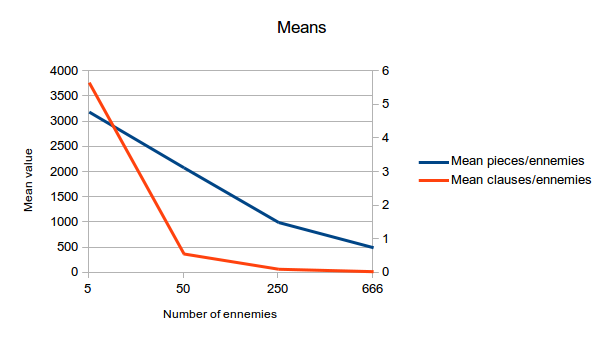
\includegraphics[scale=0.6]{mean.png}
\caption{Orange line is related to the left Y axe and blue line is related to the right one.}\end{center}
\end{figure}


As the first tabular showed, the number of clauses doesn't seems to evolve a lot related to the increasing number of ennemies. As seen in figure 1, the average number of pieces of equipments or number of clauses decreases doesn't grow as fast as the number of ennemies. We can so compute larger models without having to care about computation time. We can explain it by the fact that even if there is only a single ennemy, the model still have to know all pieces from merchant and all conflicts or abilities related to them and this is the model main part.


\end{description}




\end{document}
